\chapter{Introduction}

\begin{definition}
[Data Mining]
is the use of efficient techniques for the analysis
of very large collections of data and the
extraction of useful and possibly unexpected
patterns in data (hidden knowledge).
\ul{The goal is to extract (human-readable) knowledge and insight from raw data.}
\end{definition}
\begin{itemize}
	\item Knowledge implies we are often not just trying to solve a task
	\item Insight implies that we should infer non-obvious knowledge
	\item Human-readable implies that knowledge should be (when possible) understood by
humans: focus on interpretability!
	\item Raw data implies we'll need to clean it
\end{itemize}

\begin{figure}[htbp]
   \centering
   
   \begin{tikzpicture}[
      box/.style={rectangle, draw, rounded corners=2pt, minimum width=3cm, minimum height=1cm, align=center}
      ]


      % Central box
      \node[box, fill=red!30] (datamining) {Data Mining};
      
      % Surrounding boxes
      \node[box, fill=blue!30, above left=of datamining] (db) {Database \\ Systems};
      \node[box, fill=blue!30, above right=of datamining] (stats) {Statistics};
      \node[box, fill=blue!30, left=of datamining] (ml) {Machine \\ Learning};
      \node[box, fill=blue!30, right=of datamining] (vis) {Visualization};
      \node[box, fill=blue!30, below left=of datamining] (algo) {Algorithm};
      \node[box, fill=blue!30, below right=of datamining] (other) {Other \\ Disciplines};
      
      % Arrows
      \draw[->] (db) -- (datamining);
      \draw[->] (stats) -- (datamining);
      \draw[->] (ml) -- (datamining);
      \draw[->] (vis) -- (datamining);
      \draw[->] (algo) -- (datamining);
      \draw[->] (other) -- (datamining);
      
   \end{tikzpicture}
   \label{fig:01/DMschema}
\end{figure}



\section{Definitions}

\subsection{Knowledge Discovery Loop}
Large collections tend to be heterogeneous in source, domain, language and refinement.
The first step is to store the data, which however does not assess its heterogeneity.
Data cleaning and integration tackle this problem, so that we get integrated sources, homogenous language, and data cleared of noise and outliers.

To look for insight on the data we have to answer questions on the data as a stakeholder. We may see patterns and ask ourselves their nature.
Pattern extraction and validation lead to possible insight.
Insight may lead to noticing that some data missing may be useful, and we may want to collect it, going back at previous steps.

\begin{figure}[htbp]
   \centering
   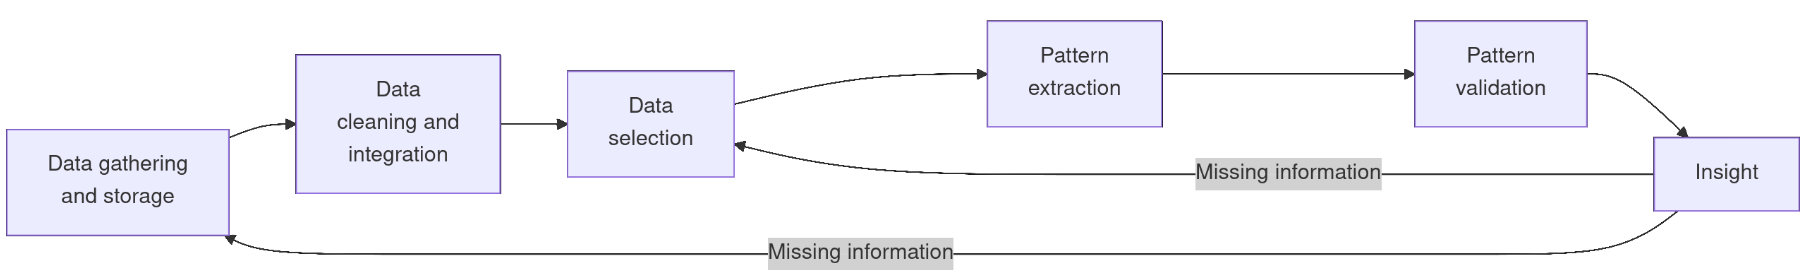
\includegraphics{images/01/knowledgeDiscoveryLoop.png}
   \caption{Knowledge Discovery Loop}
   This essentially summarizes the KDD process.
   
   \label{fig:01/knowledgeDiscoveryLoop}
\end{figure}


\subsection{KDD Process}
\begin{figure}[htbp]
   \centering
   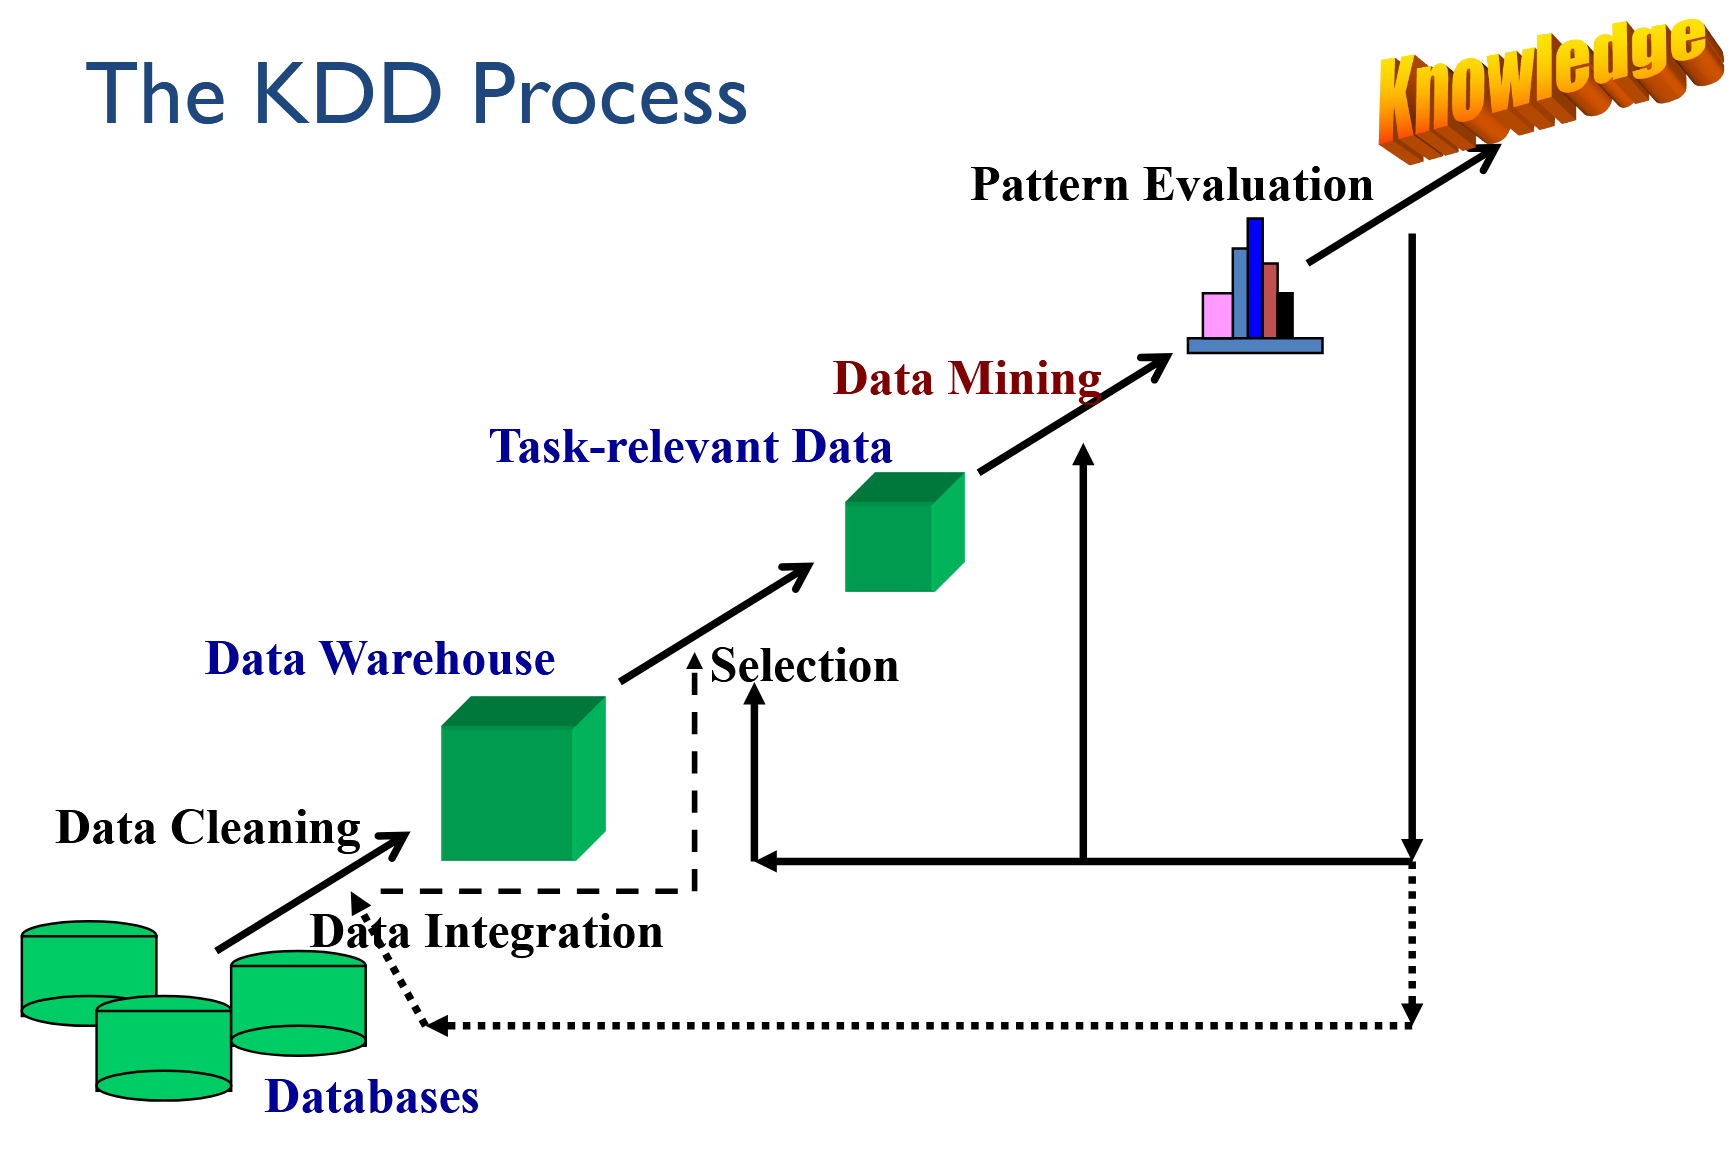
\includegraphics{images/01/KDDprocess.png}
   \caption{KDD Process}
   \label{fig:01/KDDprocess}
\end{figure}

The KDD process consists of the following steps:
\begin{enumerate}
      \item \textbf{Data Cleaning:} Remove noise and inconsistent data.
      \item \textbf{Data Integration:} Combine multiple data sources.\\
      Involves the process of data understanding, data cleaning, merging data coming from multiple sources and transfoming them to load them into a \textbf{Data Warehouse}.\\
      \textbf{Data Warehouse} is a database targeted to answer specific business questions
      \item \textbf{Data Selection:} Select relevant data for analysis.
      \item \textbf{Data Transformation:} Transform data into suitable formats for mining (summary, aggregation, etc.).
      \item \textbf{Data Mining:} Apply algorithms to extract patterns.
      \begin{itemize}
         \item \textit{Prediction Methods}\\
          Use some variables to predict unknown or future values of other variables.
         \item \textit{Description Methods}\\
          Find human-interpretable patterns that describe the data.
      \end{itemize}
      \item \textbf{Pattern Evaluation:} Identify truly interesting patterns.
      \item \textbf{Knowledge Presentation:} Present the mined knowledge in an understandable way.
\end{enumerate}

\subsection{Data Mining Process}
\begin{figure}[htbp]
   \centering
\begin{tikzpicture}[
    box/.style={rectangle, draw, minimum width=3cm, minimum height=1cm, align=center},
    annobox/.style={rectangle, rounded corners=6pt, draw, minimum width=4cm, align=center},
    textnode/.style={align=left}
]

% Main flow
\node[textnode] (input) {Input\\Data};
\node[box, right=1.5cm of input] (preproc) {Data \\ Preprocessing};
\node[box, right=2cm of preproc] (mining) {Data \\ Mining};
\node[box, right=2cm of mining] (postproc) {Postprocessing};
\node[textnode, right=2cm of postproc] (info) {Information};

% Arrows main flow
\draw[-{Latex[length=3mm,width=2mm]}, thick] (input) -- (preproc);
\draw[-{Latex[length=3mm,width=2mm]}, thick] (preproc) -- (mining);
\draw[-{Latex[length=3mm,width=2mm]}, thick] (mining) -- (postproc);
\draw[-{Latex[length=3mm,width=2mm]}, thick] (postproc) -- (info);

% Rounded-rectangle annotation for Preprocessing
\node[annobox, below=1.2cm of preproc] (prebox) {Feature Selection\\Dimensionality Reduction\\Normalization\\Data Subsetting};
\draw[-] (prebox.north) -- (preproc.south);

% Rounded-rectangle annotation for Postprocessing
\node[annobox, below=1.2cm of postproc] (postbox) {Filtering Patterns\\Visualization\\Pattern Interpretation};
\draw[-] (postbox.north) -- (postproc.south);

\end{tikzpicture}
   \label{fig:01/DMprocess}
\end{figure}


\begin{definition}
[Primary Data]
Original data that has been collected for a specific purpose.\\
Primary data is not altered by humans
\end{definition}

\begin{definition}
   [Secondary Data]
   Data that has been already collected and made available for other purposes.\\
   Secondary data may be obtained from many sources
\end{definition}

\begin{figure}[htbp]
   \centering
   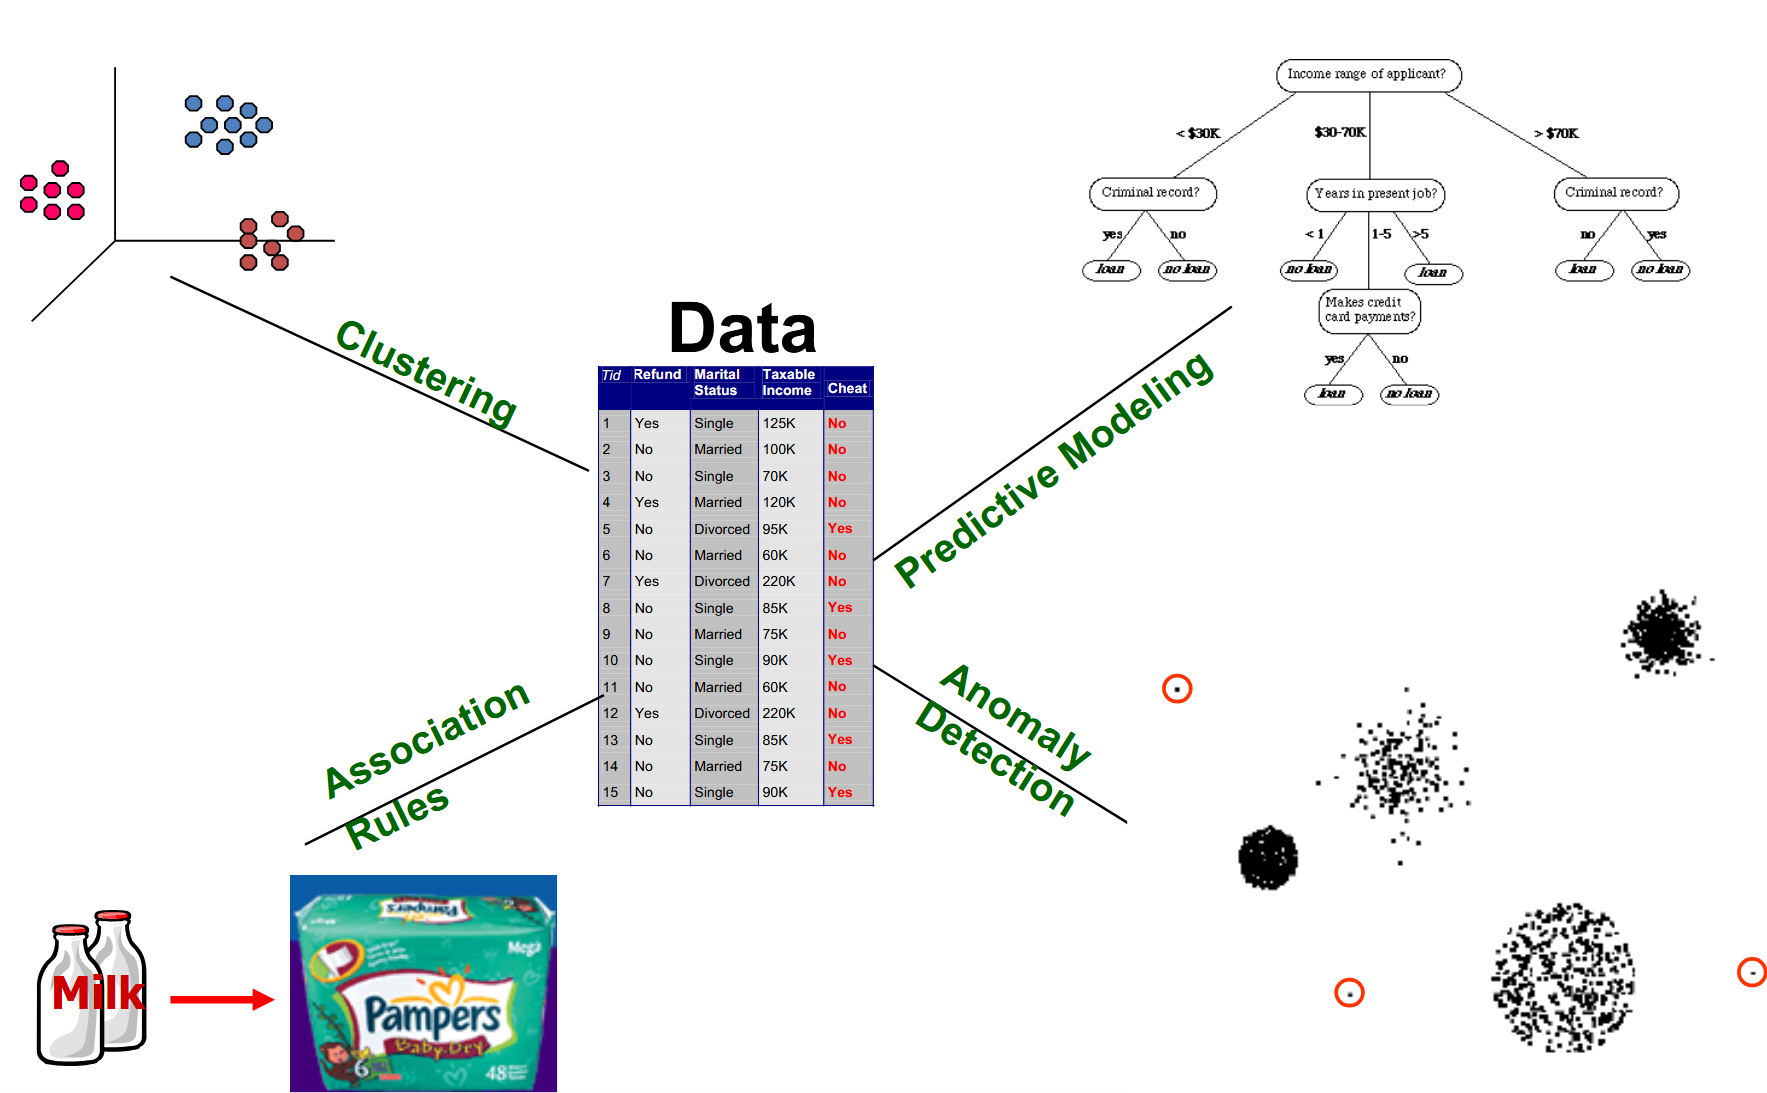
\includegraphics{images/01/datamining.png}
   \caption{Data Mining methods}
   \label{fig:01/datamining}
\end{figure}

\begin{figure}[htbp]
   \centering
   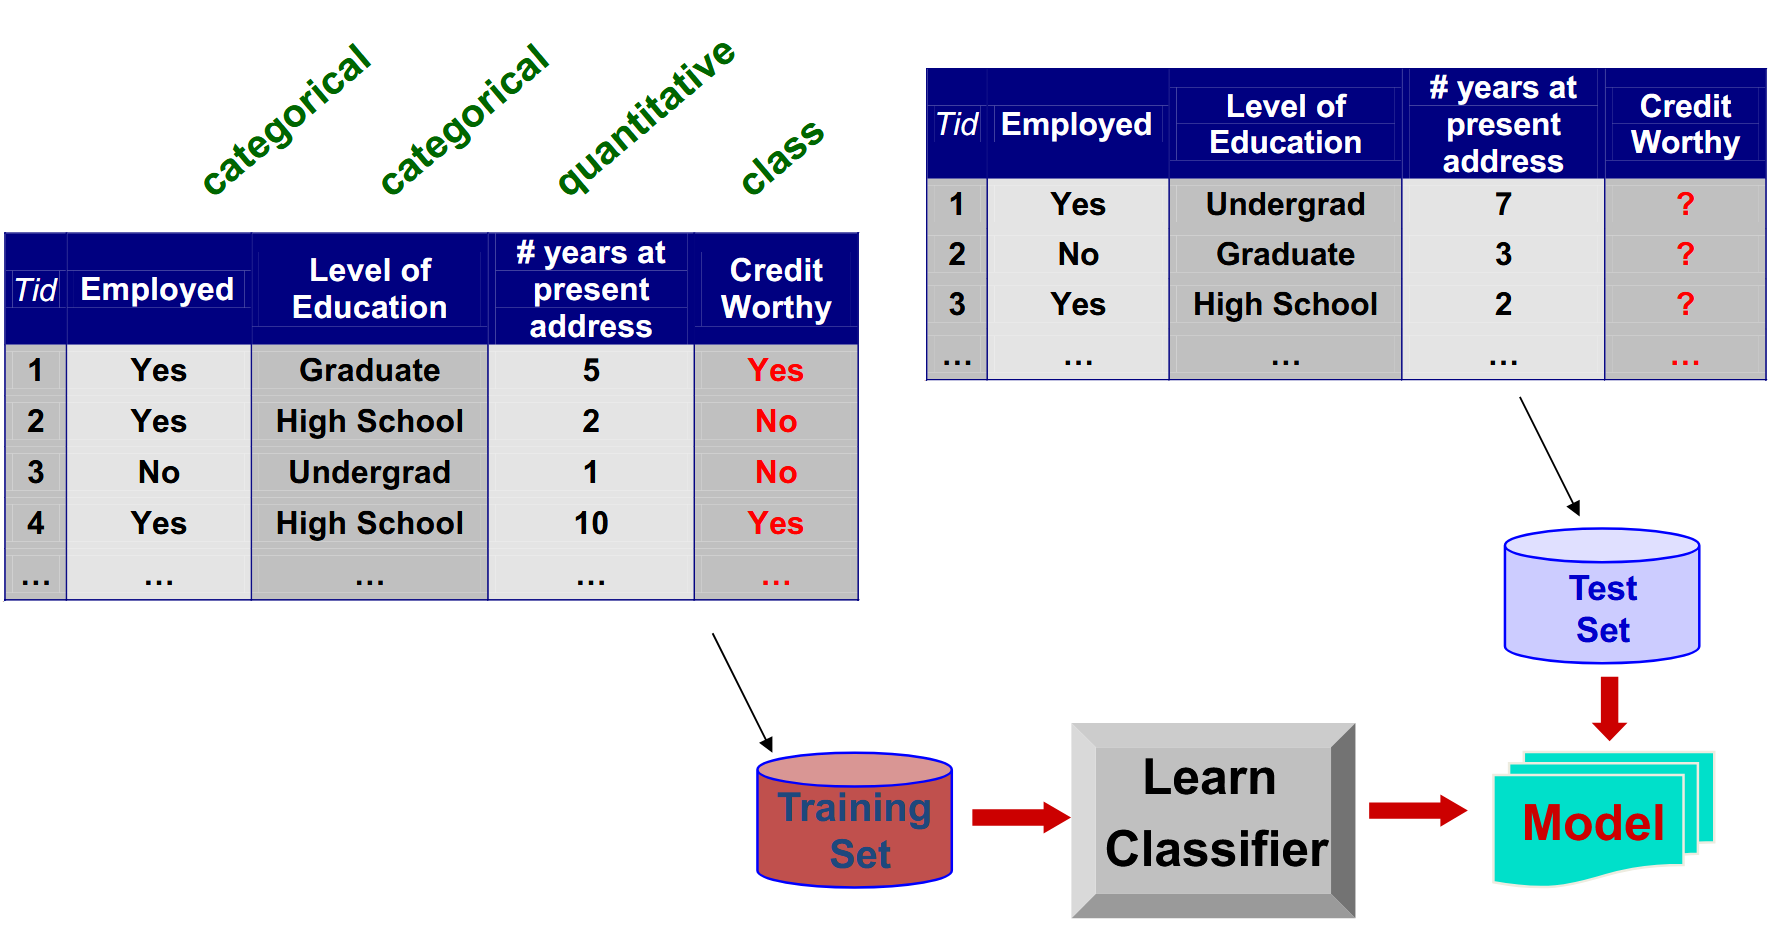
\includegraphics{images/01/classificationProcess.png}
   \caption{Classification Process}
   \label{fig:01/classificationProcess}
\end{figure}

\begin{definition}
   [Association rule discovery]
   Given a set of records each of which contain some number of items from a given collection.\\
   Produce dependency rules which will predict occurrence of an item based on occurrences of other items.
\end{definition}


\framedt{Association Use Cases}{
   \begin{itemize}
      \item \textbf{Market-basket analysis}\\
      Rules are used for sales promotion, shelf management,
      and inventory management
      \item \textbf{Telecommunication alarm diagnosis}\\
      Rules are used to find combination of alarms that occur
      together frequently in the same time period
      \item \textbf{Medical Informatics}\\
      Rules are used to find combination of patient symptoms
      and test results associated with certain diseases
   \end{itemize}
}

\section{Data Understanding}

\begin{definition}
   [Data]
   Data is a collection of data objects and their attributes.\\
   An attribute is a property or
   characteristic of an object. 
   A collection of attributes
   describe an object (record).
\end{definition}

If data objects have the same fixed set of numeric attributes,
then the data objects can be thought of as points in a multi-dimensional space, where each dimension represents a distinct
attribute.\\
Such data set can be represented by an $m\times n$ matrix, where there are m rows, one for each object, and n columns, one for each attribute.

{Data Types:\ns
\begin{itemize}
   \item Document data
   \item Transaction data
   \item Graph data
   \item Ordered data
   \begin{itemize}
      \item Spatial data
      \item Temporal data
   \end{itemize}
\end{itemize}}

{The type of the attribute depends on the following properties:\ns
\begin{itemize}
   \item Distinctness: $= \neq$
   \item Order: $< >$
   \item Differences are meaningful: $+ -$
   \item Ratios are meaningful: $* /$
\end{itemize}}

{Attribute types:\ns
\begin{itemize}
   \item Nominal/Categorical: attribute values in a finite domain (\textit{distinctness})
   \item Binary: special case of nominal with two values
   \item Ordinal: attribute values have a total ordering (\textit{distinctness} and \textit{order})
   \item Numeric: quantity (integer or real-valued) (\textit{distinctness}, \textit{order}, \textit{differences})
   \item Ratio-Scaled: we can speak of values as being an order of magnitude larger than the unit of measurement (\textit{all 4 properties})
   \note{length, counts, elapsed time (A baseball game lasting 3 hours is 50\% longer than a game lasting 2 hours)}
   \item Discrete/Continuous: attribute values are discrete (finite or countably infinite) or continuous (real-valued).
\end{itemize}}

% Attribute tab here
 \begin{table}[h!]
\centering
\rowcolors{2}{cyan!10}{white}
\begin{tabular}{p{2.7cm}p{4.2cm}p{4.2cm}p{3.2cm}}
\rowcolor{cyan!30}
	extbf{Attribute Type} & \textbf{Description} & \textbf{Examples} & \textbf{Operations} \\
Nominal & Nominal attribute values only distinguish. ($=, \neq$) & zip codes, employee ID numbers, eye color, sex: \{male, female\} & mode, entropy, contingency correlation, $\chi^2$ test \\
Ordinal & Ordinal attribute values also order objects. ($<, >$) & hardness of minerals, \{good, better, best\}, grades, street numbers & median, percentiles, rank correlation, run tests, sign tests \\
Interval & For interval attributes, differences between values are meaningful. ($+, -$) & calendar dates, temperature in Celsius or Fahrenheit & mean, standard deviation, Pearson's correlation, $t$ and $F$ tests \\
Ratio & For ratio variables, both differences and ratios are meaningful. ($*, /$) & temperature in Kelvin, monetary quantities, counts, age, mass, length, current & geometric mean, harmonic mean, percent variation \\
\end{tabular}
\caption{Attribute types, examples and operations}
\end{table}

\section{Data Understanding - Lab}

Data comes from diverse sources, and generally is not tailor-made for some downstream task. We need to start from basics:
\begin{itemize}
	\item What features are available?
	\item What are they measuring, exactly?
	\item What properties do they have?
	\item What are their relations?
	\item Are there outliers?
	\item \dots
\end{itemize}

Data can be of different nature which may co-occur:
\begin{itemize}
	\item \textbf{Temporal}: the data describes events over time
	\item \textbf{Sequential}: the data spans some ordering
	\item \textbf{Relational}: the data describes event in between instances
	\item \textbf{Spatial}: the data describes space
	\item \textbf{Independent}: instances in data are independent observations
\end{itemize}

\subsection{Data Collections}
We refer to single instances in the collections as objects/records/instances, which are
described by attributes.

\begin{table}[h!]
\centering
\begin{tabular}{ccccc}
\toprule
\textbf{Id} & \textbf{Age} & \textbf{Income} & \textbf{Marital} & \textbf{Loan} \\
\midrule
0 & 30 & 2.5k & Married & Yes \\
1 & 24 & 1.4k & Single  & No  \\
\ldots & \ldots & \ldots & \ldots & \ldots \\
\bottomrule
\end{tabular}
\caption{Grant Data}
\end{table}

\begin{itemize}
	\item Attributes: \lstinline|Id , Age , Income , Marital,Loan grant|
	\item Records: \lstinline|0, 30, 2.5k, Married, Yes , 1, 24,1.4k, Single, No|
\end{itemize}

\subsection{Data Types}
\subsubsection{Tabular}
When records are independent, and described by the same finite set of features, they
are often represented in a tabular form: the data matrix. Each row is a record, each
dimension is an attribute.


Records on the rows, attributes on the columns.

\begin{table}[h!]
\centering
\begin{tabular}{ccccccc}
\toprule
\textbf{Id} & \textbf{Age} & \textbf{Bike used} & \textbf{Length} & \textbf{Duration} & \textbf{Date} & \textbf{Cyclist} \\
\midrule
0 & 28 & Colnago VRS4 & 152.4 & 3:43:12 & 15-5-2025 & Alessandro Covi \\
1 & 40 & Cervelo RS5  & 72.4  & 2:55:01 & 4-3-2024  & Gianni Affino  \\
\bottomrule
\end{tabular}
\caption{Cyclist Data}
\end{table}

\subsubsection{Transaction}
A feature contains a (multi)set of items.

\begin{table}[h!]
\centering
\begin{tabular}{ccc}
\toprule
\textbf{PurchaseId} & \textbf{Cart} & \textbf{Bought on} \\
\midrule
0 & Bread, Milk & 17:12-15-5-2025 \\
1 & Notebook, Pens, Bread, Basil & 8:04-4-3-2024 \\
\bottomrule
\end{tabular}
\caption{Transaction Data}
\end{table}

Records on the rows, attributes on the columns.

\subsubsection{Graph}
\begin{figure}[htbp]
   \centering
   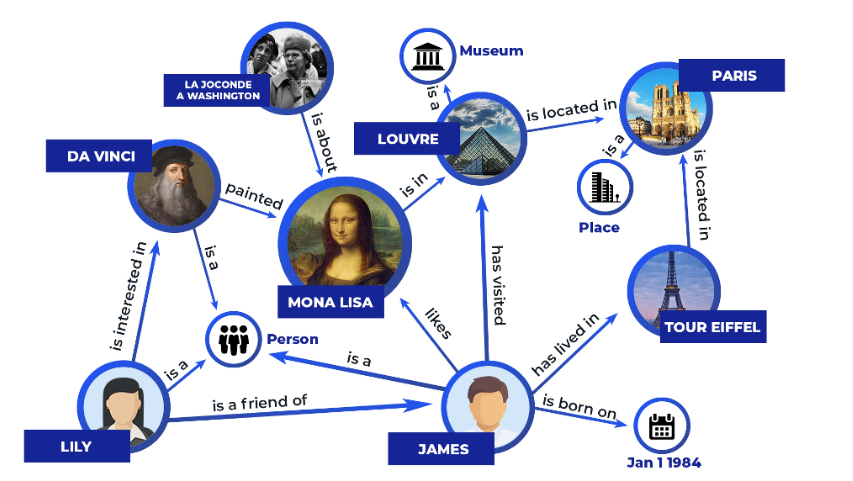
\includegraphics{images/01/graph.png}
   \caption{Graph Data}
   \label{fig:01/graph}
\end{figure}
Data is linked, either on records or features.
Records are nodes in a graph, attributes can vary wildly across records.

\newpage
\subsubsection{Sequential}
\begin{paracol}{2}
   Records are sequences (of variable length): attributes are indexed (order or time).
   

   \note{Image on the right lacks two images \smiley}
   \switchcolumn
   
   \begin{figure}[htbp]
      \centering
      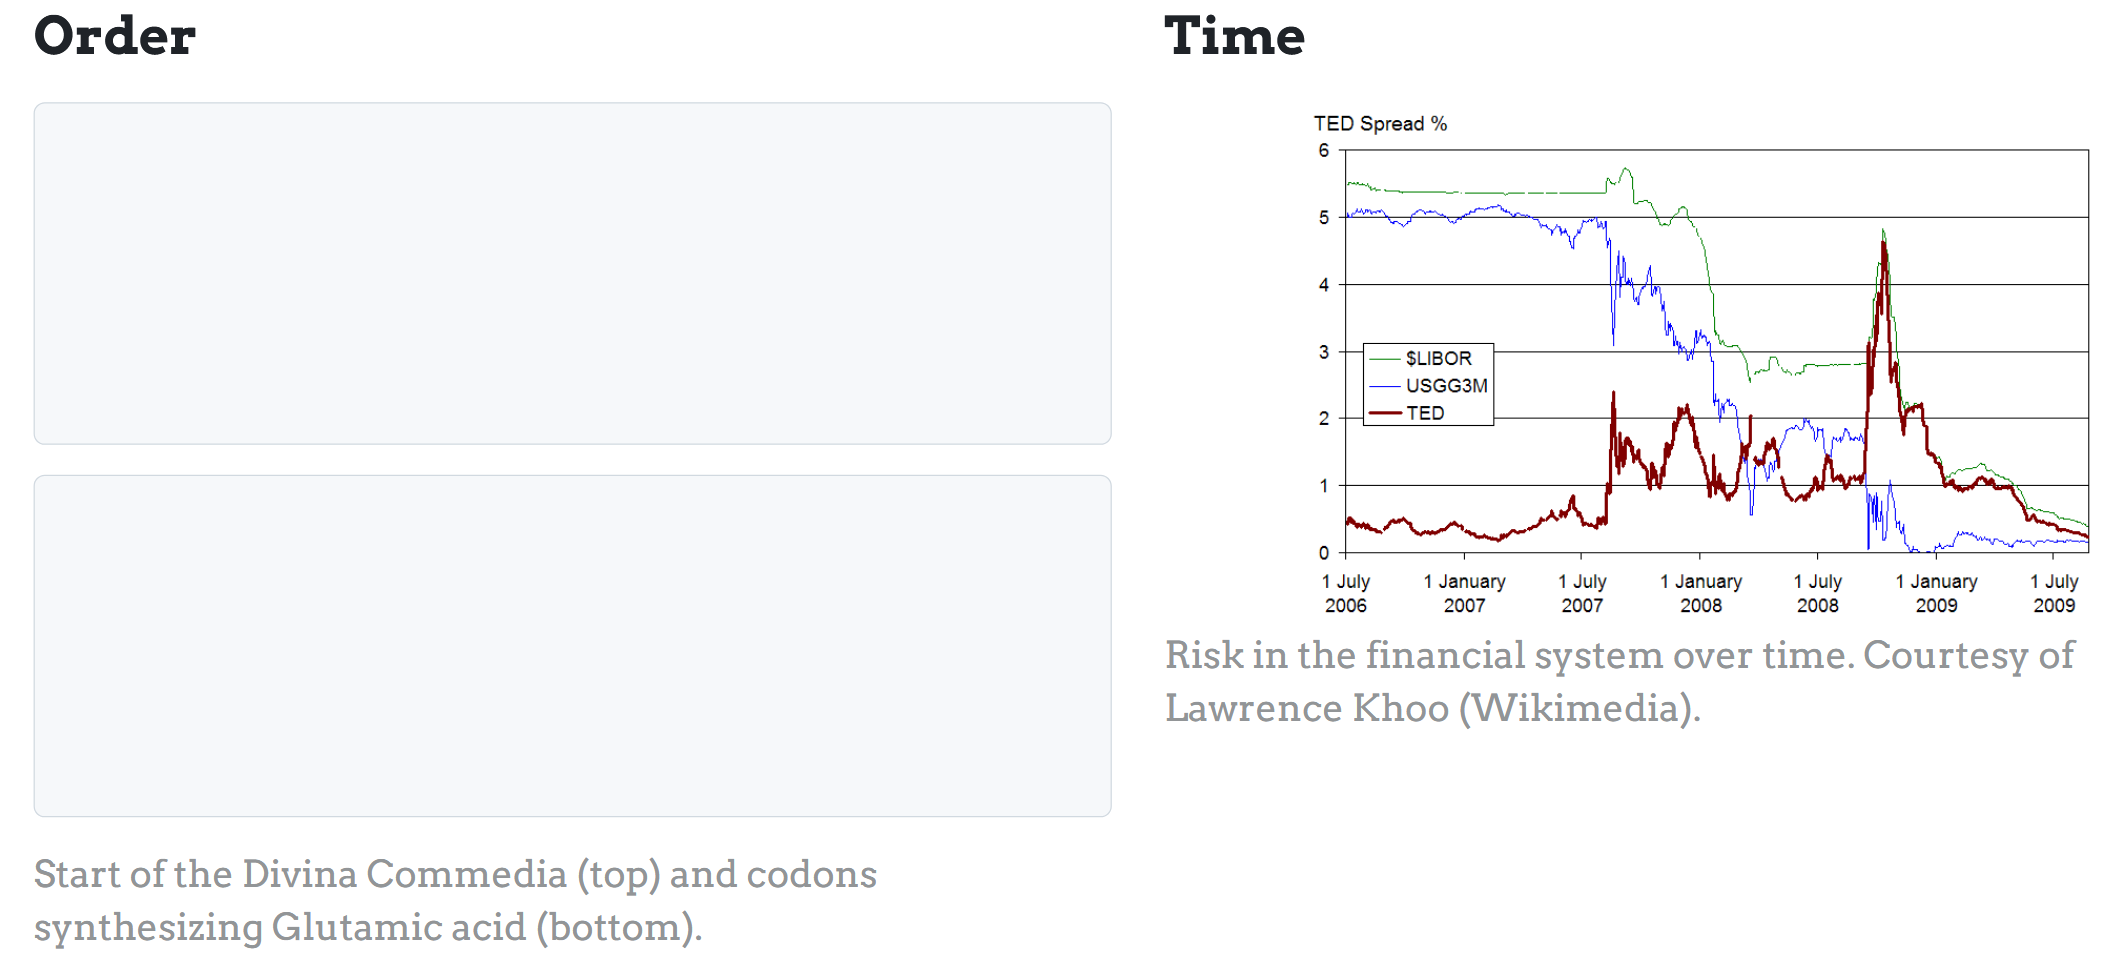
\includegraphics{images/01/sequential.png}
      \caption{Sequential Data}

      \label{fig:01/sequential}
   \end{figure}
\end{paracol}

\subsubsection{Spatial}
\begin{paracol}{2}
   

   Records are associated with locations in space: attributes can include coordinates, regions, etc.
   \switchcolumn
   
   \begin{figure}[htbp]
      \centering
      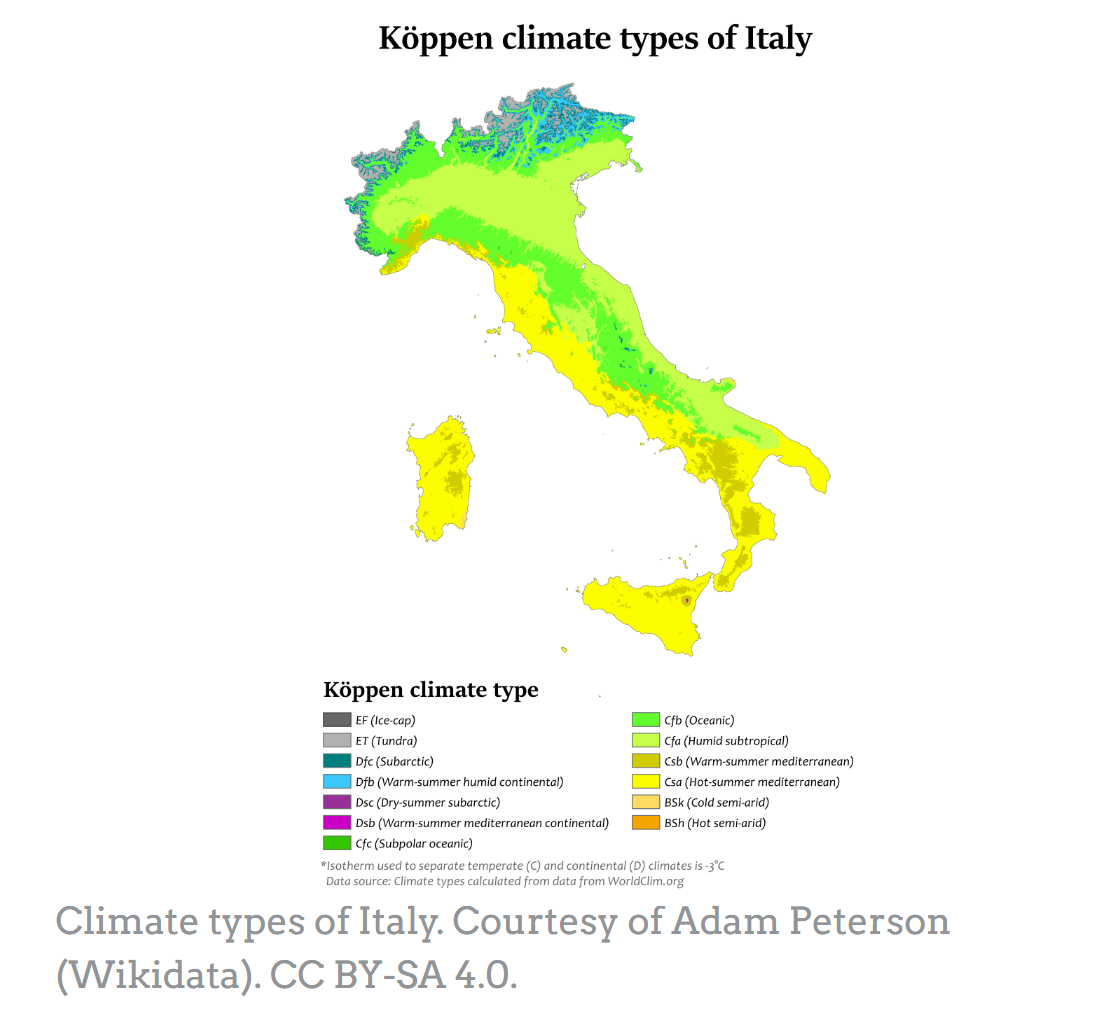
\includegraphics{images/01/spatial.png}
      \caption{Spatial Data}
      \label{fig:01/spatial}
   \end{figure}
\end{paracol}

\subsubsection{Attribute types}
\begin{table}[h!]
\centering
\rowcolors{2}{gray!10}{white} % alterna righe grigio/bianco
\begin{tabular}{lll}
\toprule
\textbf{Type} & \textbf{Description} & \textbf{Example} \\
\midrule
\textbf{Numerical}   & Values have a total ordering, and represent some numerical quantity & Age, dates \\
\textbf{Ordinal}     & Values have a total ordering, and represent some quantity           & Dress size, Cup size \\
\textbf{Binary}      & Values are one of two categories: no ordering                       & Boolean values \\
\textbf{Categorical} & Values of one of multiple categories: no ordering                   & Country, Job \\
\bottomrule
\end{tabular}
\caption{Types of Data}
\end{table}

\subsubsection{Values types}
Values can be either:
\begin{itemize}
   \item \textbf{Discrete}
   Defined in a finite or countably finite domain, e.g., country, job, cup size. Note: ordinal values may be discrete too!
   \item \textbf{Continuous}
   Defined in a continuous and infinite domain, e.g., distance.
\end{itemize}

\subsection{Data Syntax and Semantics}

\begin{paracol}{2}
   
   Given the categorization of the records and attributes of your data, we can study its
   general behavior. We leverage some basic statistical tools, first of all by drawing the
   empirical distribution of the attributes.
   
   \switchcolumn

   \begin{figure}[htbp]
      \centering
      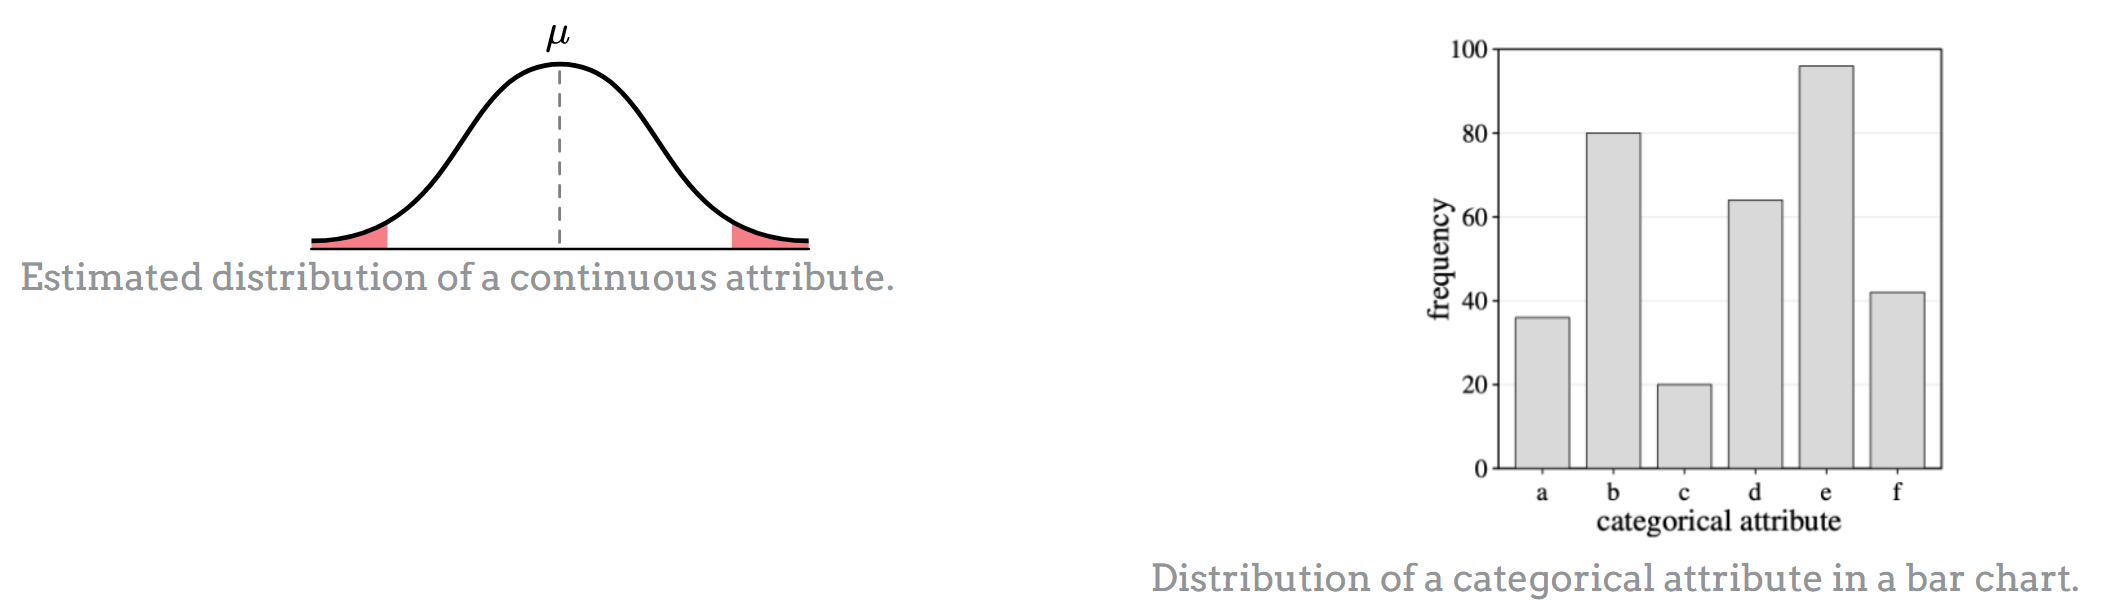
\includegraphics{images/01/semantics.png}
      \caption{Data Syntax and Semantics}
      \label{fig:01/semantics}
   \end{figure}

\end{paracol}

\framedt{Useful statistics for data semantics}{
 \begin{itemize}
 	\item \textbf{Expected value}
 	      \[
 		      \mathbb{E}[X] = \sum_{x \in \mathrm{dom}(X)} \Pr(X = x)\, x
 	      \]
 	      A statistic
 	      representative of
 	      the value of an
 	      attribute, weighing
 	      values and their
 	      probability
 	\item \textbf{Variance}
 	      \[
         \sigma^2(X) = \mathbb{E}\left[ \sum_{x \in \mathrm{dom}(X)} \big(x - \mathbb{E}[X]\big)^2 \right]
         \]
 
 	      Distance from the
 	      expected value of
 	      all records: the data
 	      spread
 	\item \textbf{Quantiles}
 	      \[
 		      q^p = x \;\; s.t.\;\; \Pr(X \leq x) = q^p
 	      \]
 	      Inflection points
 	      defining values for
 	      a threshold, e.g., if
 	      the 99-th percentile
 	      is , then we
 	\item \textbf{Interquantile range}
 	      \[
 		      q^{75} - q^{25}
 	      \]
 	      Distance between
 	      quantiles: how
 	      spread are
 	      inflection points?
 \end{itemize}
}

\begin{figure}[htbp]
   \centering
   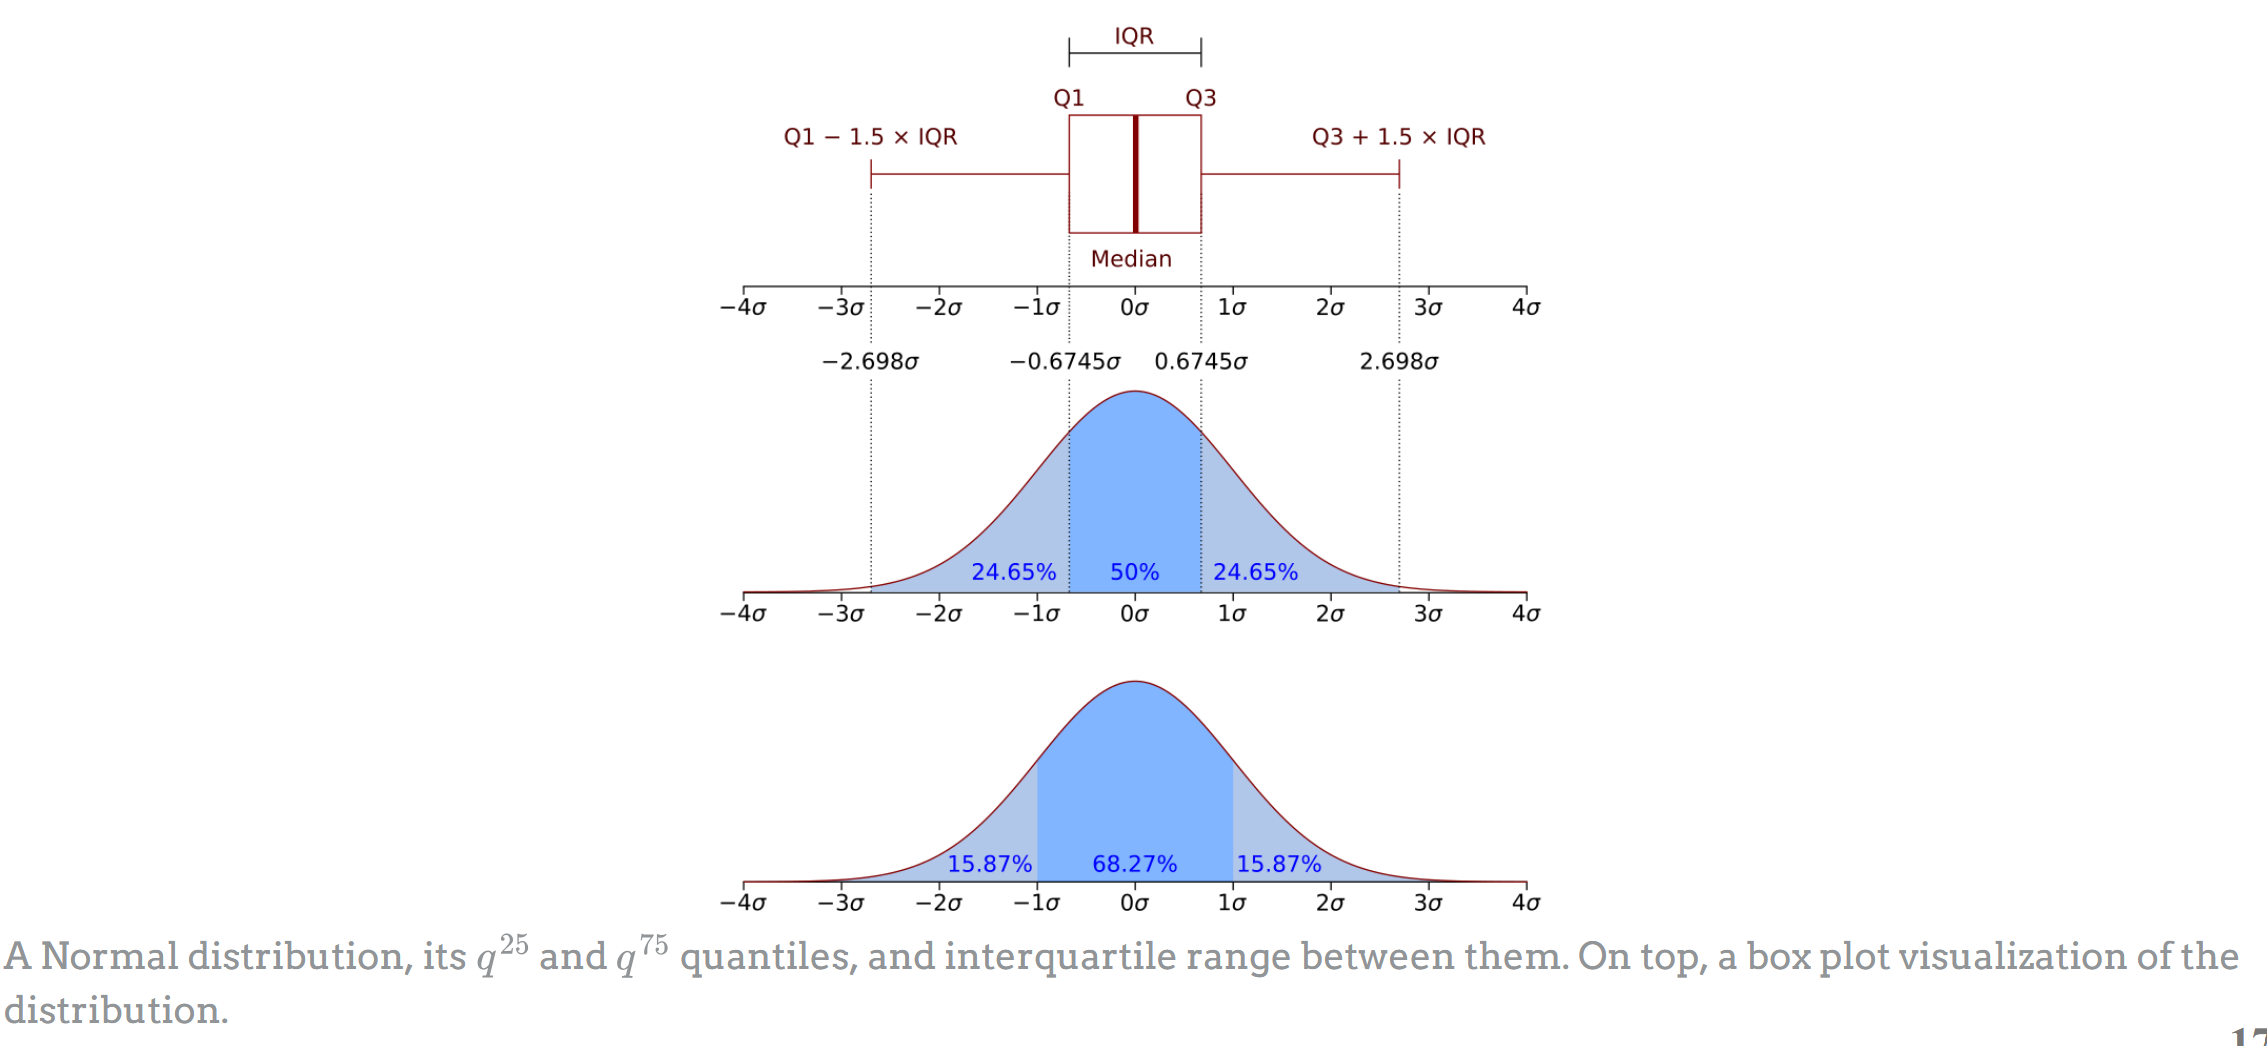
\includegraphics{images/01/statisticsgraph.png}
   \caption{Statistics Graph}
   \label{fig:01/statistics}
\end{figure}

Statistical summary of the distribution are typically accompanied by visual and semantic one.\\
\ul{Erroneous or weird values to be cleaned later may already pop up in these basic steps.}
Outlier values typically skew statistics. Variance is often replaced by absolute/median average deviation

\section{Data Cleaning}

There are some concepts to be aware of when dealing with data quality, hence data cleaning.
\nl

\textbf{Data accuracy} is the degree to which data correctly describes the "real world" object or event being
described.
\begin{itemize}
	\item Syntactic: values outside domain, e.g., Eataly in Country
	\item Semantic: values in domain, but semantically wrong, e.g., age is 3, and weight is 82kg
\end{itemize}

\textbf{Completeness} is the degree to which all required data is known.\\
Some attributes are not collected, or are collected partially, e.g., temperature was not
recorded by the sensor.

\textbf{Biased gathering} is the degree to which data may be over/under-representative, e.g., the bank may only provide data about successful loan applicants.

\textbf{Timeliness} is the degree to which data is up to date.


Remember: \textit{garbage in, garbage out!}\footnote{i.e. if you have garbage data, you'll get garbage results} In a task-agnostic view, we are interested in addressing the above by tackling:
\begin{itemize}
	\item \textbf{Duplicates}: skews the data distribution
	\item \textbf{Missing values}: give false/partial information
	\item \textbf{Noise}: uninformative of the data
	\item \textbf{Poor accuracy}: gives wrong data
	\item \textbf{Outliers}: skews the data distribution and models of the data
\end{itemize}

\subsection{Handling Duplicates}
Remove them... when appropriate! Not all duplicates are garbage, it depends on what insight you can gather from it.
\begin{paracol}{2}
\textbf{Case A}\\
You have data on registration to your
website, with several duplicate e-mails.
Insights:
\begin{itemize}
	\item The ``Sign in'' button is hard to find
	\item The ``Sign in'' button is less visible
	      than the ``Sign up'' button
	\item Your site is so anonymous people
	      forget they signed up already
\end{itemize}
\switchcolumn
\textbf{Case B}\\
You have data on credit account opening
from Poste (Italian postal service) with
several duplicate e-mails.
Insights:
\begin{itemize}
	\item The client hacked the database and
	      added themselves to ask more
	      credit (unlikely)
	\item Poste's tech staff is underwhelming (very likely)
\end{itemize}
\end{paracol}

\subsubsection{Duplicate Features}
Duplicate features may be more tricky. Features convey similar, although not equal, information to others.\\
Examples:
\begin{itemize}
	\item Resting heart rate and heart rate under
continuous high effort
	\item Education level and reading skills
	\item Rent and available bank deposit
\end{itemize}
These pairs of features are not per se one duplicate
of the other, but are strongly related: when one
grows, so does the other, and when one goes down,
so does the other.
\nl

Linear (and rank) relationships between two features $X,Y$ can be quantified with their
correlation. Correlation ranges in \([-1, 1]\), from perfectly negative to perfectly positive
correlation.\\
Given two lists of values $x^{i^n},y^{i^n}$ we can compute two main correlation types.
\begin{itemize}
   \item \textbf{Pearson correlation}
         \[
            \rho_P^{X,Y} = \frac{\mathbb{E}\left[(x^i - \mathbb{E}[X])(y^i - \mathbb{E}[Y])\right]}{\sigma_X \sigma_Y}
         \]
         Measures linear correlation between two numerical features and their values.
   \item \textbf{Spearman correlation}
         \[
            \rho_S = \rho_P^{\text{rank}(X), \text{rank}(Y)}
         \]
         Measures monotonic correlation between two ordinal or numerical features.
\end{itemize}

\subsection{Handling Missing Values}
Data may be missing for any number of reasons (at random or not at random).
\begin{itemize}
	\item A record has a large and/or significant set of missing attributes
	\item An attribute has a large percentage of missing values
\end{itemize}
We have two choices: \textbf{dropping} or \textbf{imputing}.

\begin{paracol}{2}
\textbf{Dropping}\\
If a record has a large and/or significant set of missing attributes, or an attribute has a
large percentage of missing values, we can drop the record/attribute.
\begin{itemize}
	\item High percentage of missing
values
	\item Missing values in critical
attributes, e.g., a patient in
cardiology has no heart rate data
\end{itemize}

\switchcolumn

\textbf{Imputing}\\
Imputing means replacing the missing value with a
``best guess'' value.\\
If a record has a small set of missing attributes, or an attribute has a small percentage of
missing values, we can impute the missing values.
We have to create a model to predict the missing value.

\begin{itemize}
	\item Low percentage of missing values
	\item Reasonably good understanding of the attribute semantics/distribution
	\item Presence of related attributes
\end{itemize}
\end{paracol}

\subsection{Outliers}

Quantiles and distributions inform us on what values may be outlier. 
They are typically dropped, and unlike missing values, almost never imputed.
We'll tackle algorithms later in the course.

\subsubsection{Flower Example}

There is a dataset with 5 attributes: sepal length, sepal width, petal length, petal width, and species (type).

\begin{table}[h!]
\centering
\begin{tabular}{ccccc}
\toprule
\textbf{Sepal L.} & \textbf{Sepal W.} & \textbf{Petal L.} & \textbf{Petal W.} & \textbf{Type} \\
\midrule
5.1 & 3.5 & 1.4 & 0.2 & Setosa \\
7.0 & 3.2 & 4.7 & 1.4 & Versicolor \\
\ldots & \ldots & \ldots & \ldots & \ldots \\
\bottomrule
\end{tabular}
\caption{Flower Dataset Example}
\end{table}

\begin{figure}[htbp]
   \centering
   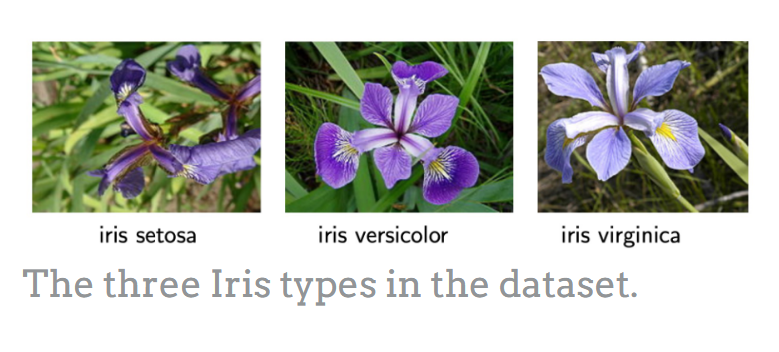
\includegraphics{images/01/flowers.png}
   \caption{Flower Data plotted}
   \label{fig:01/flower}
\end{figure}

\begin{figure}[htbp]
   \centering
   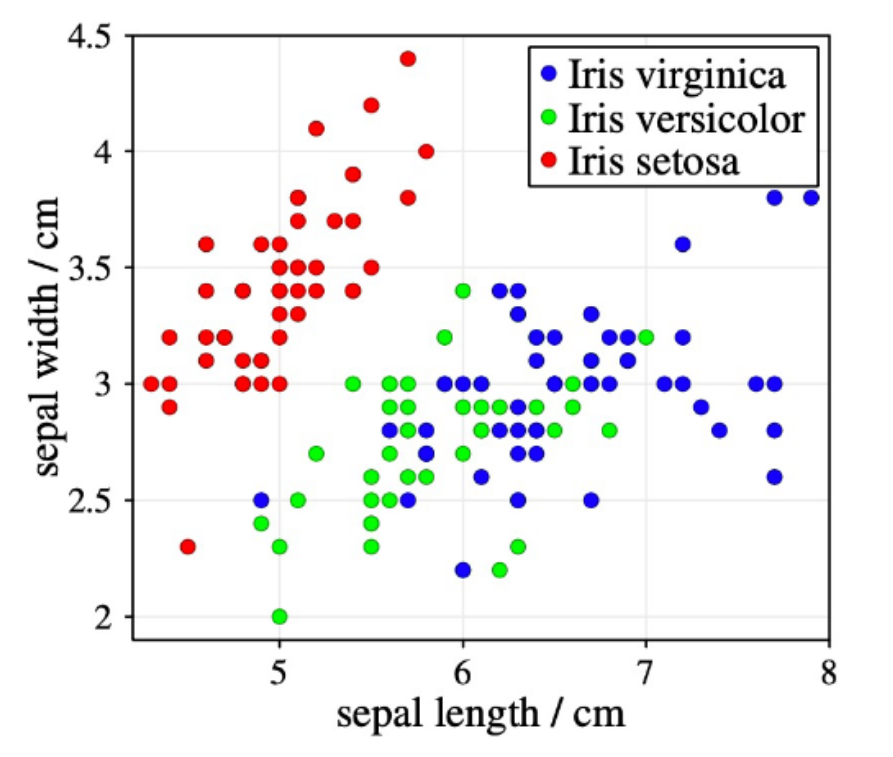
\includegraphics[width=0.49\columnwidth]{images/01/scatterplot.png}
   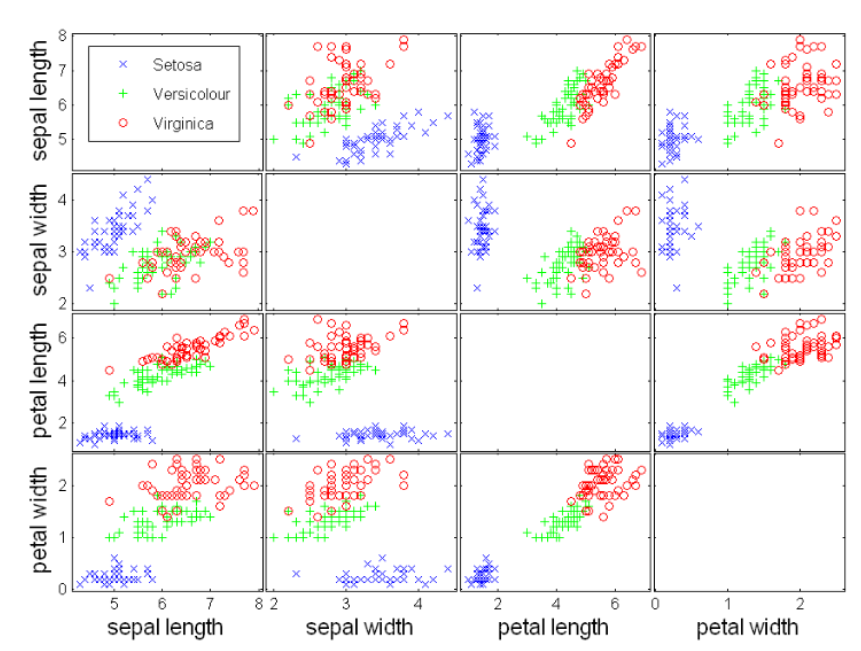
\includegraphics[width=0.49\columnwidth]{images/01/scattermatrix.png}
   \caption{Scatter plot of sepal length and width, and scatter matrix: scatter plots of all pairs of attributes in the Iris dataset.}

   Plot bivariate (or trivariate) data, eyeing data correlation and outliers.
   \label{fig:01/scatterplot}
\end{figure}



\section{Data Preparation}
We will delve into the following techniques of data preparation:
\begin{itemize}
	\item Aggregation
	\item Data Reduction: Sampling
	\item Dimensionality Reduction
	\item Feature subset selection
	\item Feature creation
	\item Discretization and Binarization
	\item Attribute Transformation
\end{itemize}

\subsection{Aggregation}
Aggregation is the process of combining two or more attributes (or objects) into a single attribute (or object).
\labelitemize{\textbf{\textit{Purpose}}}{
	\begin{itemize}
		\item Data reduction\\
		      \begin{itemize}
			      \item Reduce the number of attributes or objects
		      \end{itemize}
		\item Change of scale\\
		      \begin{itemize}
			      \item Cities aggregated into regions, states, countries, etc.
			      \item Days aggregated into weeks, months, or years
		      \end{itemize}
		\item More “stable” data\\
		      \begin{itemize}
			      \item Aggregated data tends to have less variability
		      \end{itemize}
	\end{itemize}
}

\subsection{Reduction}
Reduction is simply reducing the amount of data
We may reduce the number of \textbf{records} by sampling or clustering, or the number of \textbf{attributes} (\textit{columns}) by selecting a subset of them, or by creating a new ---smaller--- set of attributes from the old one.

\subsubsection{Sampling}
Sampling is the main technique employed for data
reduction.\\
It is often used for both the preliminary investigation of the data and the final data analysis.

Sampling is typically used in data mining because
processing the entire set of data of interest is too
expensive or time consuming.

{The key principle for effective sampling is the
following:\ns
\begin{itemize}
	\item Using a sample will work almost as well as using the entire
	      data set, if the sample is representative
	\item A sample is representative if it has approximately the same
	      properties (of interest) as the original set of data
\end{itemize}
}

\begin{itemize}
   \item  \textbf{Simple Random Sampling}
   \begin{itemize}
   	\item There is an \textit{equal probability} of selecting any particular item
	\item Sampling \textbf{without replacement}
   \begin{itemize}
   	\item As each item is selected, it is removed from the population
   \end{itemize}
	\item Sampling \textbf{with replacement}
   \begin{itemize}
   	\item Objects are not removed from the population as they are
   selected for the sample.
	\item In sampling with replacement, the same object can be picked
   up more than once
   \end{itemize}
   \item \textbf{Stratified sampling}
	\item Split the data into several partitions; then draw random samples
   from each partition
	\item Approximation of the percentage of each class
	\item Suitable for distribution with peaks: each peak is a \textbf{layer}
   \end{itemize}
\end{itemize}

\begin{figure}[htbp]
   \centering
   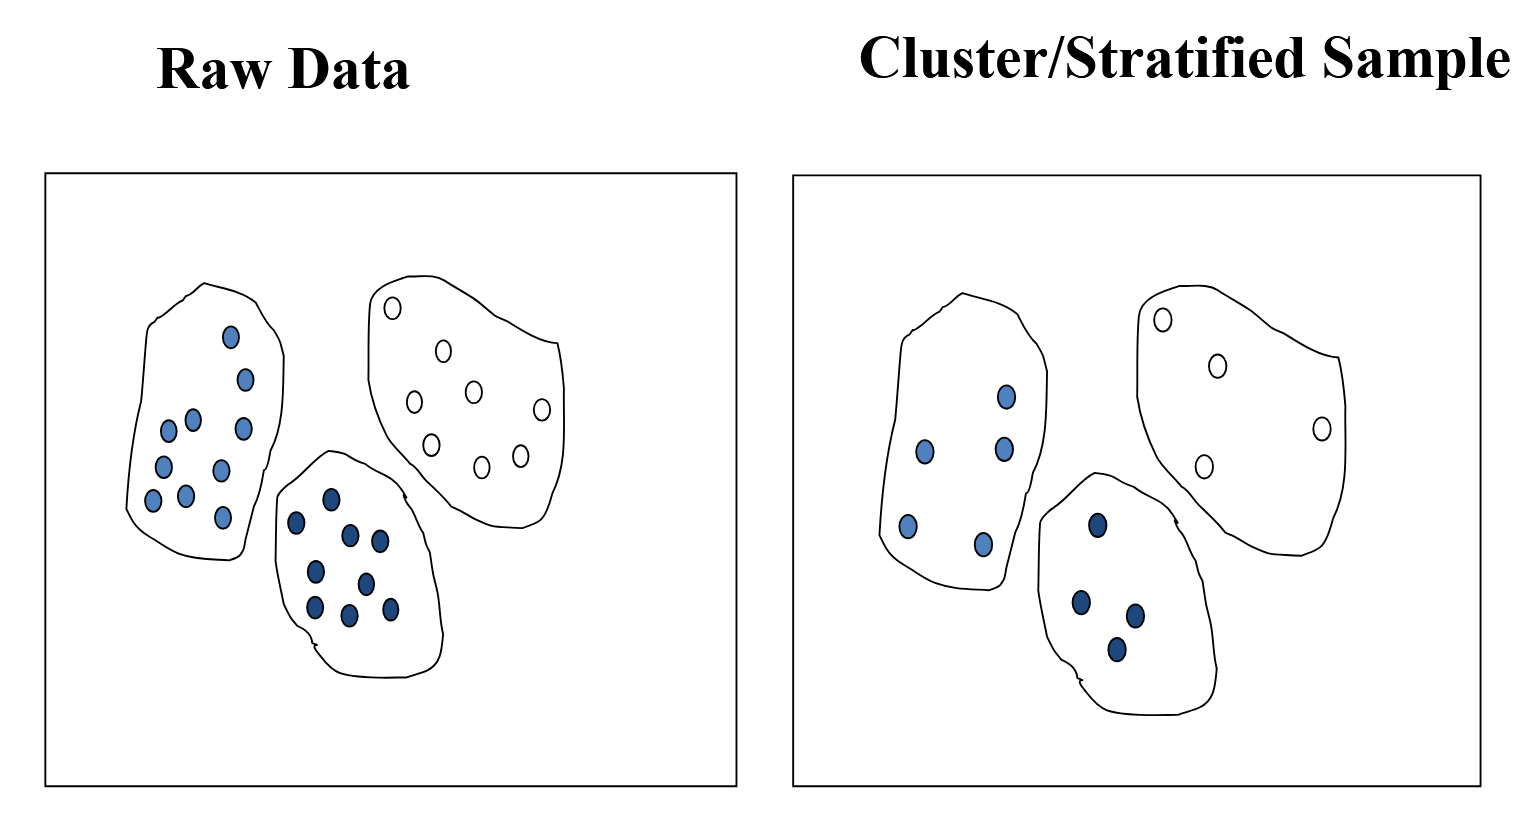
\includegraphics{images/01/stratifiedSampling.png}
   \caption{Stratified Sampling}
   \label{fig:01/stratifiedSampling}
\end{figure}

\subsubsection{Dimensionality Reduction}
This consists in reducing the number of attributes (or features) in the data.
We want a selection of a subset of attributes that is as small as possible and sufficient for the data analysis.
\begin{itemize}
	\item removing (more or less) irrelevant features
\begin{itemize}
	\item Contain no information that is useful for the data mining
task at hand
	\item Example: students' ID is often irrelevant to the task of
predicting students' GPA
\end{itemize}
	\item removing redundant features
\begin{itemize}
	\item Duplicate much or all of the information contained in one or
more other attributes
	\item Example: purchase price of a product and the amount of
sales tax paid
\end{itemize}
\end{itemize}

\framedt{Curse of Dimensionality}{
   When dimensionality increases, data becomes \textbf{increasingly sparse} in the space that it occupies.

   Definitions of density and distance between points, which are critical for clustering and outlier detection, become less meaningful.

   This phenomenon is known as the \textbf{curse of dimensionality}.
   }
   \begin{figure}[htbp]
      \centering
      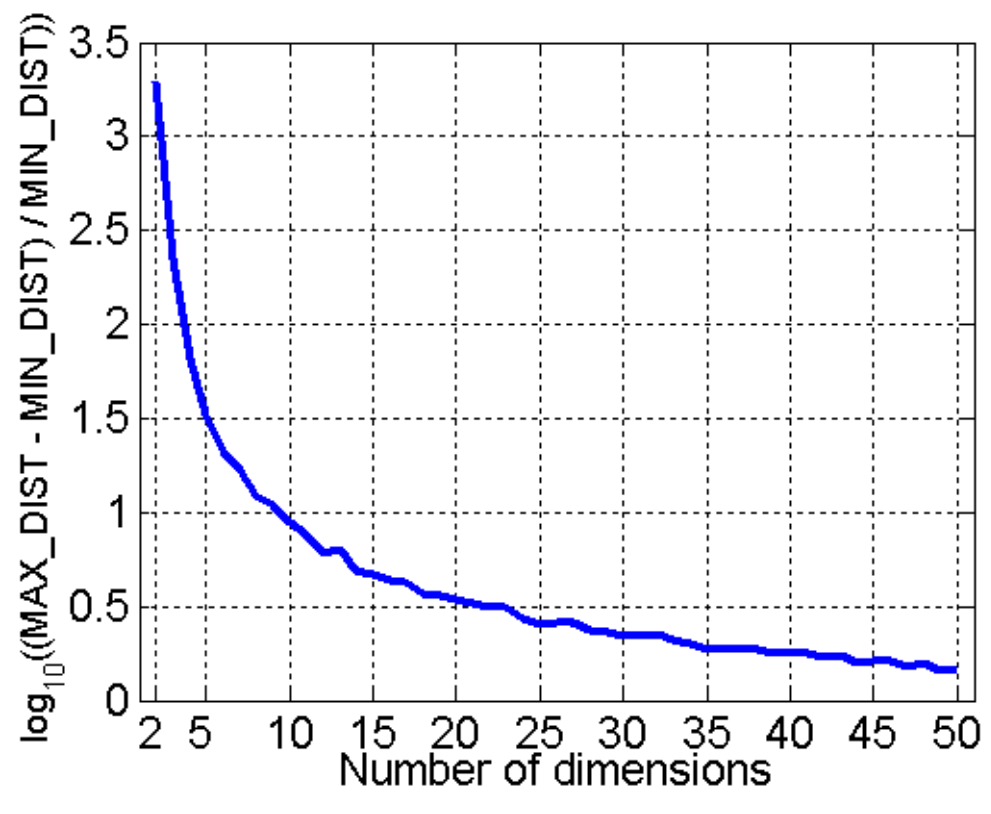
\includegraphics{images/01/dimensionalitycurse.png}
      \caption{$log_{(MAXDIST-MINDIST)/MINDIST}$ decreases as the dimensionality increases, meaning that the difference between the farthest and nearest neighbor distances becomes less significant}
      \label{fig:01/dimensionalitycurse}
   \end{figure}


{Purposes of dimensionality reduction include:\ns
\begin{itemize}
	\item Avoid curse of dimensionality
	\item Reduce amount of time and memory required by data
mining algorithms
	\item Allow data to be more easily visualized
	\item May help to eliminate irrelevant features or reduce noise
\end{itemize}}

{Techniques to do so include:\ns
\begin{itemize}
	\item Principal Components Analysis (PCA)
	\item Singular Value Decomposition
	\item Others: supervised and non-linear techniques
\end{itemize}}

\subsubsection{Feature Subset Selection}
Feature subset selection consists in selecting a subset of the original features.
The goal is to find a minimal subset of features that is as good as the entire set of features for the data analysis task at hand.

For removing irrelevant features, it is needed a \textbf{performance measure} indicating how well a feature
or subset of features performs w.r.t. the considered
data analysis task.

For removing \textbf{redundant features}, either a
\textit{performance measure} for subsets of features or a
\textit{correlation measure} is needed.

\textbf{Filter Methods}
\begin{itemize}
	\item Selection after analyzing the \textbf{significance} and \textbf{correlation} with other
attributes
	\item Selection is independent of any data mining task
	\item The operation is a pre-processing
\end{itemize}
\textbf{Wrapper Methods}
\begin{itemize}
	\item Selecting the top-ranked features using as reference a DM task
	\item Incremental Selection of the ``best'' attributes
	\note{``Best'' = with respect to a specific measure of statistical significance (e.g.: information gain)}
\end{itemize}
\textbf{Embedded Methods}
\begin{itemize}
	\item Selection as part of the data mining algorithm
	\item During the operation of the DM algorithm, the algorithm itself decides which attributes to use and which to ignore (e.g. Decision tree)
\end{itemize}

\framedt{Feature Selection Techniques}{
	\begin{itemize}
		\item \textbf{Selecting the top-ranked features}: Choose the features with
		      the best evaluation when single features are evaluated.
		\item \textbf{Selecting the top-ranked subset}: Choose the subset of
		      features with the best performance. This requires exhaustive
		      search and is impossible for larger numbers of features. (For 20
		      features there are already more than one million possible
		      subsets.)
		\item \textbf{Forward selection}: Start with the empty set of features and
		      add features one by one. In each step, add the feature that yields
		      the best improvement of the performance.
		\item \textbf{Backward elimination}: Start with the full set of features and
		      remove features one by one. In each step, remove the feature
		      that yields to the least decrease in performance.
	\end{itemize}
}